% 2018clpsych.tex - 2018 CLPsych paper

\documentclass{article}
\usepackage{times}
\usepackage{graphicx}
\usepackage{amsmath}
\usepackage{algorithm2e}
\usepackage[top=3cm, bottom=3cm, left=3cm, right=3cm]{geometry}

\begin{document}

\title{Predicting Change in a User's Risk of Self-Harm Based on Community Interaction in an Online Support Forum}
\author{
Arman Cohan, Julien Han, Nazli Goharian, Luca Soldaini, Tim Walsh\\
Georgetown University\\
}
\maketitle

\begin{abstract}
Given a large, partially labeled dataset of posts from an online mental health support forum, we present a system that predicts how users' risk of self-harm changes over a period of time based on posts made by other forum users during that period. The system uses a machine learning approach in two distinct stages. The first stage classifies all of the posts in the dataset according to users' apparent risk level. The second stage, which is the focus of this paper, then predicts users' end-state given their initial state and a set of posts directed towards them by other users. The goal is to learn how a forum community can better support users in distress by extracting feature weights from the second stage classifier. This paper shows that our system can predict users' end-states, but the extracted feature weights remain open to interpretation and raise philosophical questions about the value of this approach.
\end{abstract}

\section{Introduction and Motivation}

\paragraph{}A number of online forums exist for people to discuss mental health issues and mutually support each other. These forums may be attractive for a variety of reasons: they provide a sense of community while generally preserving anonymity and privacy; participation is essentially free compared to professional therapy; and they are continuously available, so users can participate when it is most convenient, or when they most need support, without waiting for an appointment with a therapist. A metastudy in late 2017\cite{marchant} found that nine out of 15 studies concluded that participation in a moderated, online support forum is beneficial for young people in a state of mental distress, five studies reached mixed conclusions, and one study found that forums were linked to an increase in suicidal ideation\cite{dunlop}.

\paragraph{}An obvious potential issue with support forums is that participants (including the moderators in most cases) are not trained and licensed as mental health practitioners, and thus cannot be expected to know how to best support users in distress or avoid triggering distress. We also note that any proven techniques used by mental health practioners, who generally work one-on-one and face-to-face with clients who trust them, may not translate easily to the setting of a large, free, anonymous, online forum. Therefore, we might be able to draw valuable insight by using empirical methods on a dataset from a real forum to learn how online communities can be more supportive of users in a state of distress.

\paragraph{}In 2016, the workshop on Computational Linguistics and Clinical Pyschology (CLPsych) obtained such a dataset from the ReachOut.com forum and challenged the text-mining community to classify each post according to users' apparent risk of self-harm\cite{milne}. Building on that work, we hypothesize that given a trained machine learning classifier that predicts the change in a target user's risk level, based on who interacts with that user and what they write, we can extract the most predictive features from the classifier to find words, phrases, topics, and other patterns that are most correlated with increased or decreased risk.

\section{Related Work}

\paragraph{}Some of the earliest work related to our line of inquiry comes from the sociologist David Phillips in the 1970s who identified an increase in the suicide rate of American and British populations following newspaper publicity of a suicide, and argued that the relationship between publicity and the increase was causal\cite{phillips}. Other researchers later found similar results in other parts of the world\cite{gladwell}\cite{jonas}\cite{ishii}\cite{cheng}\cite{sonneck}, across various types of media, and involving different types of subjects such as fictional characters and celebrities\cite{stack}. While this work focused on passive exposure to print or broadcast media across large populations, other research has focused on the contagion of suicide within smaller social clusters\cite{gould1}\cite{gould2}\cite{haw}\cite{brent}. All of this feeds our intuition that who interacts with a target forum user, and what other users say to them, may be predictive of the target user's risk of self-harm.

\paragraph{}The previously mentioned work focuses on the power of suggestion in a negative way, but a much larger body of research examines how to positively influence individuals who suffer from depression, suicidal thoughts, and other mental health concerns. As the very foundation of clinical psychology, we assume that readers of this paper have a better grasp of the general state-of-the-art than we can possibly present here ourselves.

\paragraph{}Some research has looked at online mental health support forums in particular, by analyzing posts or questioning users, at least in terms of how they are used and what benefits they might provide compared to their risks. However, we are not aware of any other research that specifically examines what language or patterns of interaction on a forum have the most positive or negative effects on users. Administrators of a forum must therefore rely on their own intuition and experiences to determine how to lead or moderate discussions.

\paragraph{}The work most closely related to ours comes from the aforementioned CLPsych workshop's shared task for 2016 and 2017. Moderators wanted a way to automatically label new posts, indicating the user's risk of self-harm as defined by a panel of experts, to quickly bring attention to users who need immediate support. CLPsych attracted 15 teams that submitted systems for this task, and ReachOut.com now employs some of the technology on their forum\cite{milne}\cite{cohan2}.

\paragraph{}The 2016 CLPsych workshop proceedings present details and results from the work of 15 teams using the same ReachOut.com dataset. Every team used a machine learning approach with, at a minimum, bag-of-words features and a supervised learning method based on the manually labeled subset of posts given for the task. Some teams incorporated a semi-supervised learning approach, leveraging datasets from Twitter and Reddit forums focused on depression. Teams selected many different combinations of features from the body text of each post as well as metadata associated with each post and user. Teams also used a variety of classifiers, with some in combination\cite{milne}. The top performing systems tended to focus on features from the body text, as opposed to metadata, such as token and character n-grams, part-of-speech tags, mood, sentiment, emotion, and topic. Top performing systems also used logistic regression and support vector machine classifiers. The highest performing system, by Kim et al., labeled the official test set with a macro-averaged F1 score of 0.42 and accuracy of 0.85\cite{kim}. Notably, some top performing systems included features from adjacent posts by other users in order to provide context, but this could also indicate influence by other users.

\paragraph{}In follow-up work for the 2017 CLPsych workshop, Cohan et al. improved a system to achieve a macro-averaged F1 score of 0.51 and accuracy of 0.95. Additionally, after labeling the entire dataset, Cohan et al. used their results to explore other research questions. One discovery was that most users who were active for two or more months on the forum showed improvement in their apparent mental state as measured by the label of their first and last posts\cite{cohan2}. Cohan et al. note that positive influence by the forum community is one possible cause for the improvement.

\section{Approach}

\paragraph{}Existing research shows strong results in identifying self-harm risk associated with mental health forum posts\cite{milne}. In particular, work by Cohan et al. shows a high accuracy and F1 scores of 0.95 and 0.51 in that task\cite{cohan2}. Therefore, instead of manually labeling the entire dataset, we utilize that method to assess the risk of all the posts in the dataset with high confidence. We then use these predictions to study how risk of self-harm might be influenced by other peers on the forum.

\paragraph{}We first restructure and filter the dataset to construct ``conversation sets." A conversation set consists of an original post or posts by a target user $U$ on day 0, followed by $L$ replies by other users mentioning $U$ by-name over some period of $N$ days. Note that this is distinct from the concept of a forum ``thread," which has one original post and subsequent replies that generally relate to one topic but may not directly address the original post or user at all. We then create a feature vector representation of the $L$ posts in the set, along with the label for $U$'s initial state and some additional metadata for the set. Finally, our classifier aims to predict the most severe label of $U$'s follow-up posts appearing in the week after the $N$-day period.

\paragraph{}For the parameter $N$, we experiment with values ranging from 1 to 14. At very low values of $N$, it is obvious that sets will contain fewer replies. In fact 40\% of sets at $N$ = 1 are empty while only 13\% of sets are empty at $N$ = 14. With that said, we exclude empty sets from the training data because their representation is identical. For large values of $N$, however, we believe that we begin to lose relevance. For example, it seems unlikely that things said on the forum in January would affect a user's state in December. Similarly, we also place a limit on the timing of the target user's ``follow-up posts," and we choose $N$ + 7. That is, if we do not find any follow-up posts to associate with a conversation set within a week of the $N$-day period, we remove that set. In addition to $N$-day periods, we also did some preliminary experiments with the idea of a ``conversation snapshot" which looked at two consecutive posts by the target user, agnostic of time, and the replies occurring between those posts, but we abandoned the idea after initial results were worse than conversation sets for all values of $N$.

\paragraph{}While constructing the sets, we filter out all of those sets where the target user is a moderator. Moderators are chosen for their stability and trustworthiness, and they are responsible for handling user crises, enforcing rules, and managing other administrative tasks. Moderators are also highly active, posting much more often than the average user. Therefore, we are less interested in the mental state of moderators, and removing them helps to balance the training data since nearly all moderator posts are labeled low-risk.

\paragraph{}Also while constructing converation sets, we remove block quotes written by the target user, and all occurrences of the target user's username token in each set. These last two steps ensure that the classifier trains on the identities and language of other users instead of training on anything about the target user directly.

\paragraph{}We then extract and experiment with the following features for each set: TF-IDF weighted unigrams, bigrams, and trigrams (stop words both included and removed using the NLTK list), the number of replies in the set, the number of replies by a moderator, the number of posts by the target user during the $N$-day period, an average risk score for replying users, sentiment polarity, and sentiment subjectivity. We define a risk score for a replying user as the percentage of their posts in the total dataset that were labeled higher-risk. We determine polarity and subjectivity for all of the replies lumped together using the TextBlob package\cite{textblob}

\paragraph{}After constructing the feature vectors from the conversation sets, we feed them to a classifier implemented with scikit-learn as a support vector machine with a linear kernel. Once we have the trained classifier, the weights of the word (unigram) and phrase (bigram and trigram) features indicate how strongly they relate to each case where a target user transitions from one risk level to another.

\section{Experimental Setup}

\paragraph{}To ensure the highest level of confidence in our results, we use a binary system of labeling posts and user states as either simply $green$ (low risk) or $flagged$ (higher risk, which aggregates several different labels from the original CLPsych shared task) because the Cohan et al. system succeeds in this task with an F1 score 0.92. To help ensure that errors from this first stage do not compound in the second stage, we take confidence values from the first stage classifier and filter out any post labeled with less than 70\% confidence when we need to use these labels. Additionally, error analysis uncovers consistent errors when labeling posts from one particular forum thread (``Turning negatives into positives," due to the unique premise and structure of that thread), so we filter out those posts as well.

\paragraph{}Another important detail is determining the label for the target user's initial state. If the user makes just one post on day 0, we simply take the label of that post. In the case where the user makes multiple posts on day 0, we tried three different methods of capturing their initial state. The ``absolute" method sets the initial state to be $flagged$ if any post on day 0 is $flagged$. The ``last post" method takes the label of the final post made by $U$ on day 0. The ``majority" method sets the initial state as $flagged$ if 50\% or more posts on day 0 are $flagged$. The ``absolute" method showed the best initial results, likely because it produces twice as many $flagged$ cases, giving us giving us a more balanced training set, so we performed all subsequent trials with this method.

\paragraph{}We define conversation set ``replies" with several different patterns. One is when the target user is quoted with the forum's block quote functionality. The others are the appearance of patterns such as ``Hey $U$, ..." or ``...@$U$..." in the post body text. We prefer this notion of a reply rather than using thread structure because we can be reasonably certain that the target user actually reads these posts, and our intuition is that they are much more likely to affect the target user than posts addressed to other users or nobody in particular. Our notion of a reply also captures conversation across multiple, parallel threads easily.

\paragraph{Dataset}The dataset provided by CLPsych for its 2016 shared task includes 65,755 posts from the ReachOut.com forum from July of 2012 to June of 2015. We obtain labels for the entire dataset using the 2017 Cohan et al. system.

\paragraph{Evaluation Plan}We evaluate our system with five-fold cross-validation looking at F1 score, accuracy, precision, and recall. F1 score is what we present in this paper. We separately evaluate conversation sets with a $green$ initial state, sets with a $flagged$ initial state, and all sets together (with initial state label as a feature). Working separately on sets that only begin with a $flagged$ state, for example, lets us reason more specifically about higher risk distressed users.

\paragraph{Results}We achieve our highest F1 score of 0.776 for all conversation sets at $N$ = 14, using the following features: TF-IDF unigrams and bigrams with stop words included, number of replies, and number of replies by a moderator. Adding all additional features (still including stop words) produces our next best F1 score of 0.775. We achieve our third best F1 score of 0.772 after removing stop words. In general, as $N$ ranges from 1 to 14, the F1 score ranged from about 0.65 to 0.77, but the increase is only monotonic up to about $N$ = 10, after which improvement flattens out. See Figure 1.

\begin{figure}[h!]
    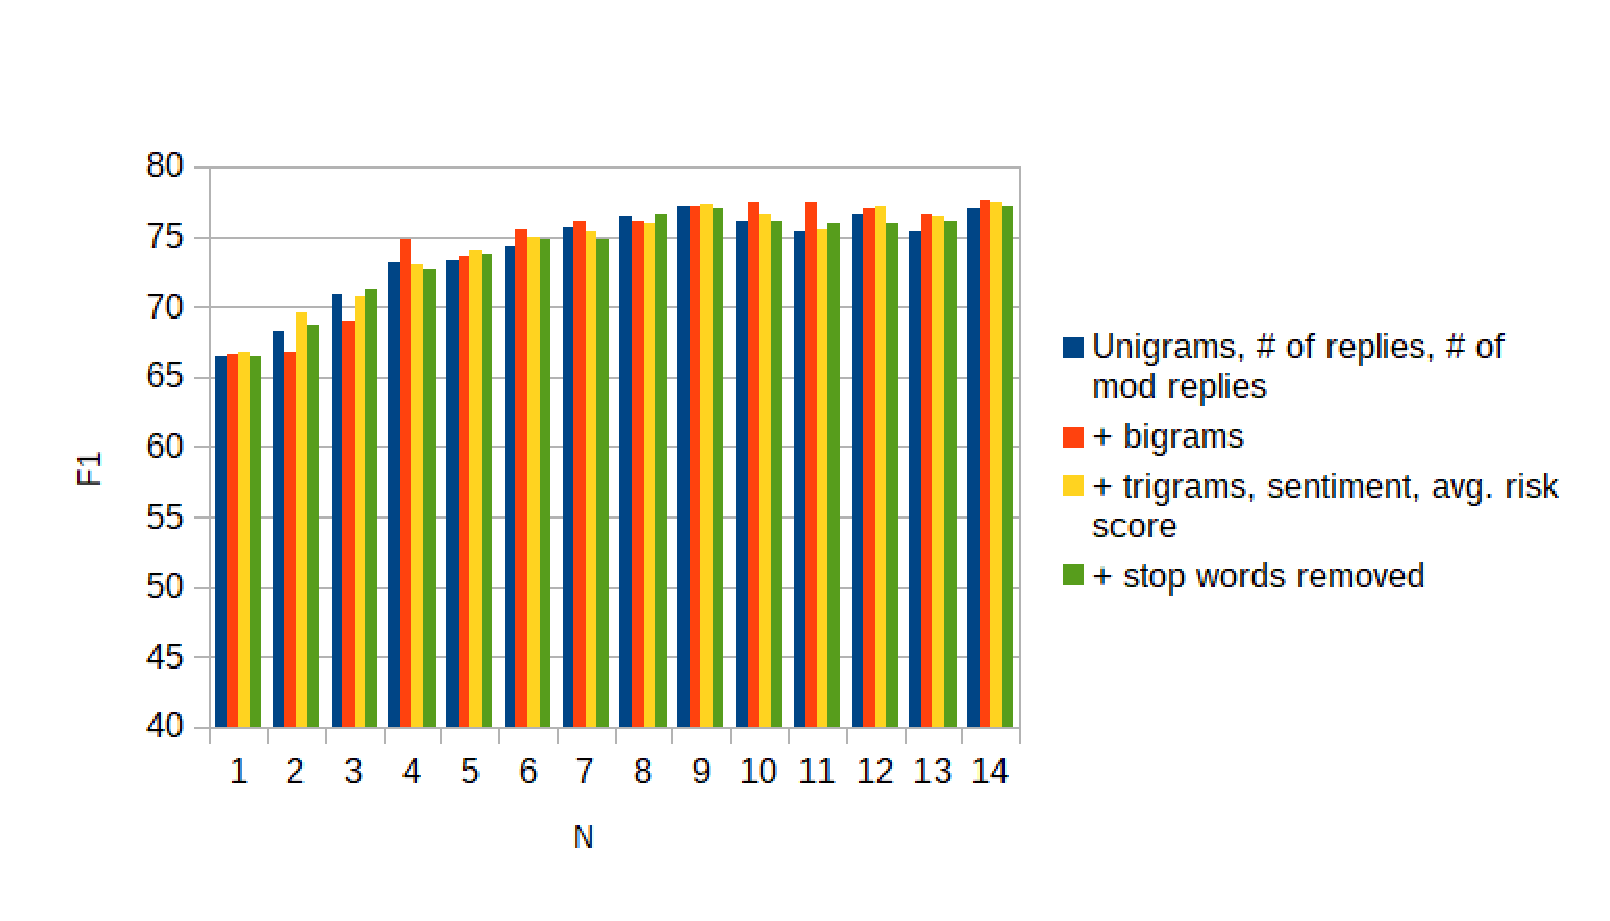
\includegraphics[width=14cm]{resultsAll}
    \caption{All Sets with Initial State Label as Feature}
\end{figure}

\subparagraph{}When the initial state is $flagged$, we achieve our highest F1 score of 0.771 at $N$ = 10, with all features and stop words included. See Figure 2.

\begin{figure}[h!]
    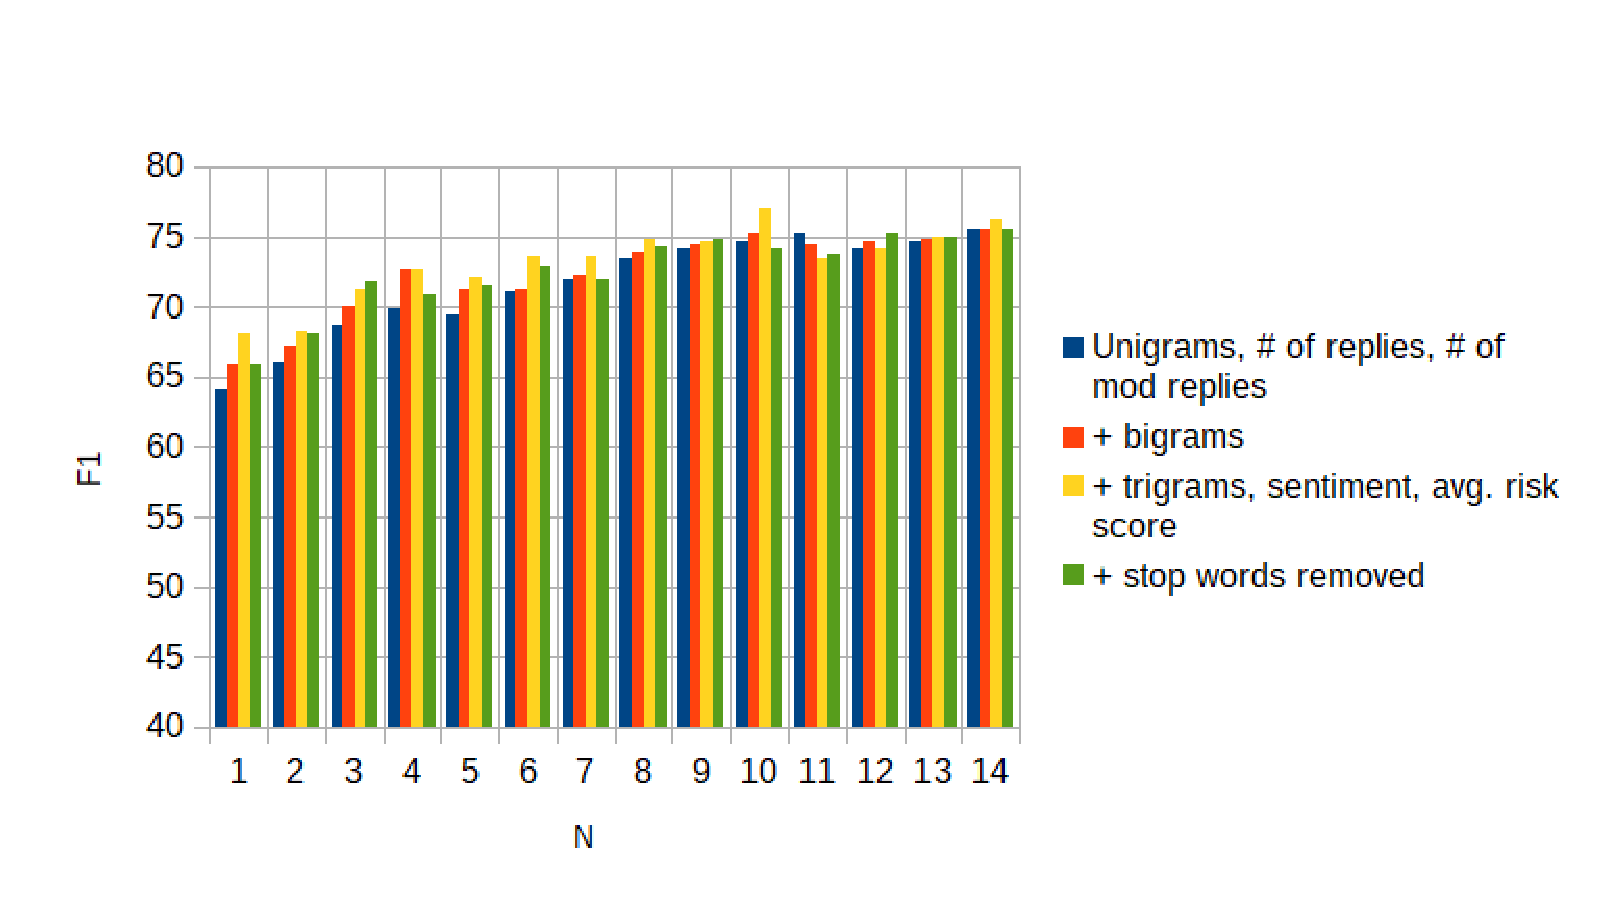
\includegraphics[width=14cm]{resultsFlagged}
    \caption{Sets with Flagged Initial State Only}
\end{figure}

\subparagraph{}When the initial state is $green$, we achieve our highest F1 score of 0.628 at $N$ = 14, with all features and stop words removed. The significantly lower score on these sets is likely explained by the extreme imbalance of the dataset. About 95\% of conversation sets with an initial state of $green$ stay $green$, compared to about 40\% of sets with an initial state of $flagged$ that stay $flagged$. See Figure 3.

\begin{figure}[h!]
    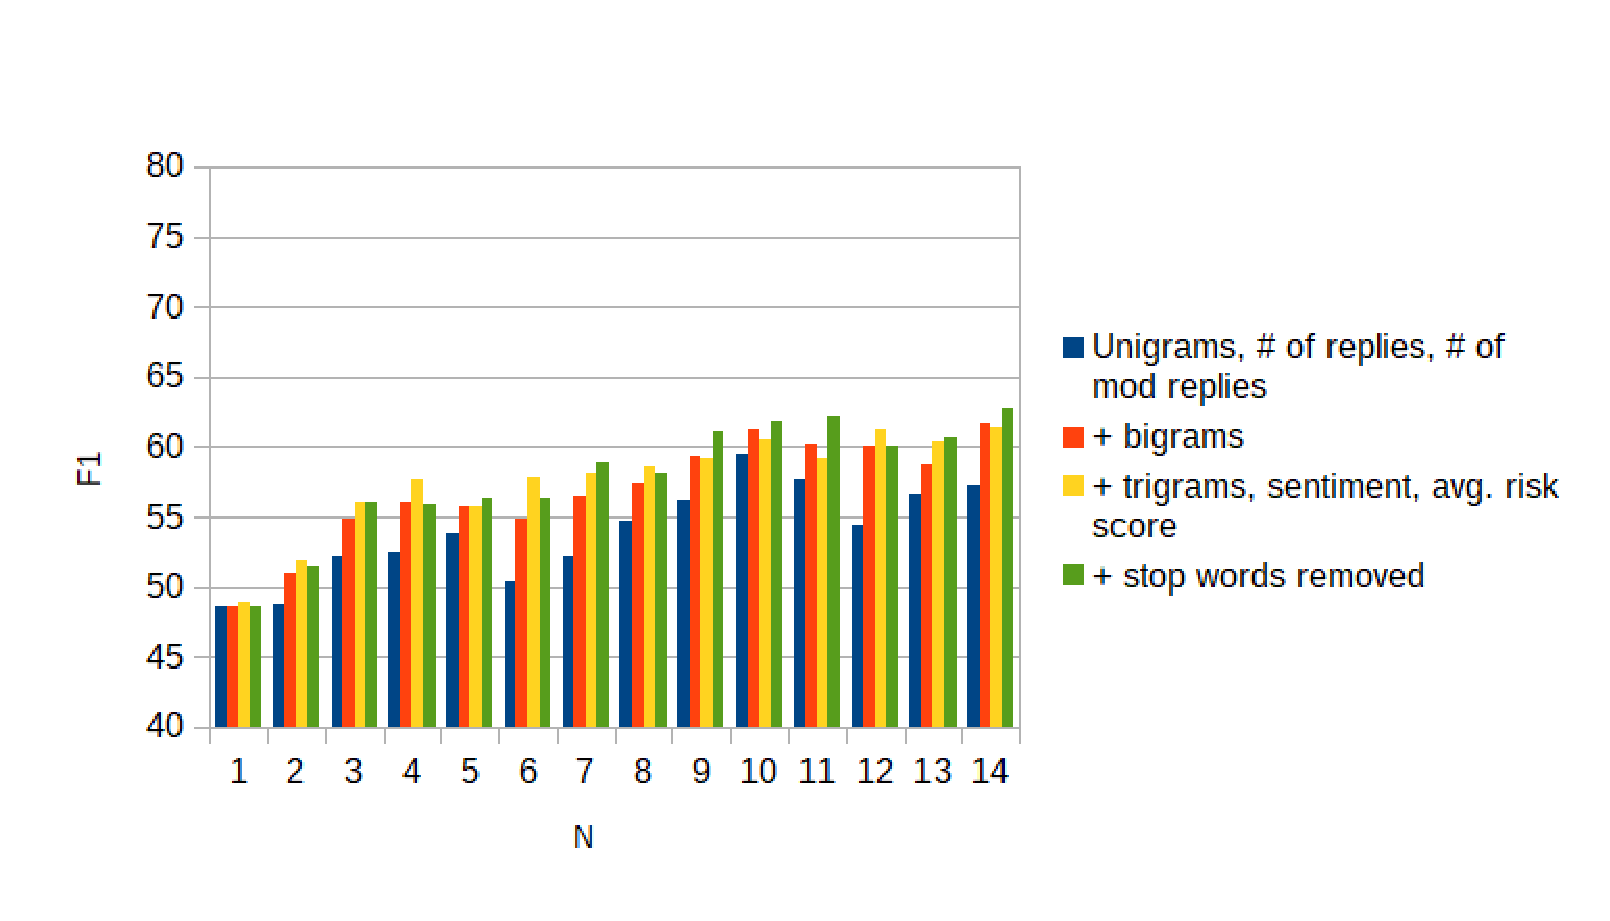
\includegraphics[width=14cm]{resultsGreen}
    \caption{Sets with Green Initial State Only}
\end{figure}

\subparagraph{}Once we have models that predict the change in target users' states reasonably well, we turn our attention to the follow-up question of how to interpret the models and gain insight into what factors might influence a target user's level of risk and how. To achieve this, we extract the top feature weights from each trained model. Here we examine the separate cases for each initial and final state label. In Figure 4, highlighted in red are (anonymized) usernames and custom features (as opposed to text N-grams). *norepliesfound* is a special token that we insert into conversation sets when they are otherwise empty. Some features stand out for their peculiarity. One is ``year 11" or ``11" which refers to the 11th grade of school in Australia, for students of age 16 or 17. Another is ``jaw" which shows up in a number of posts talking about TMJ pain, associated with grinding or clenching teeth.

\begin{figure}[h!]
    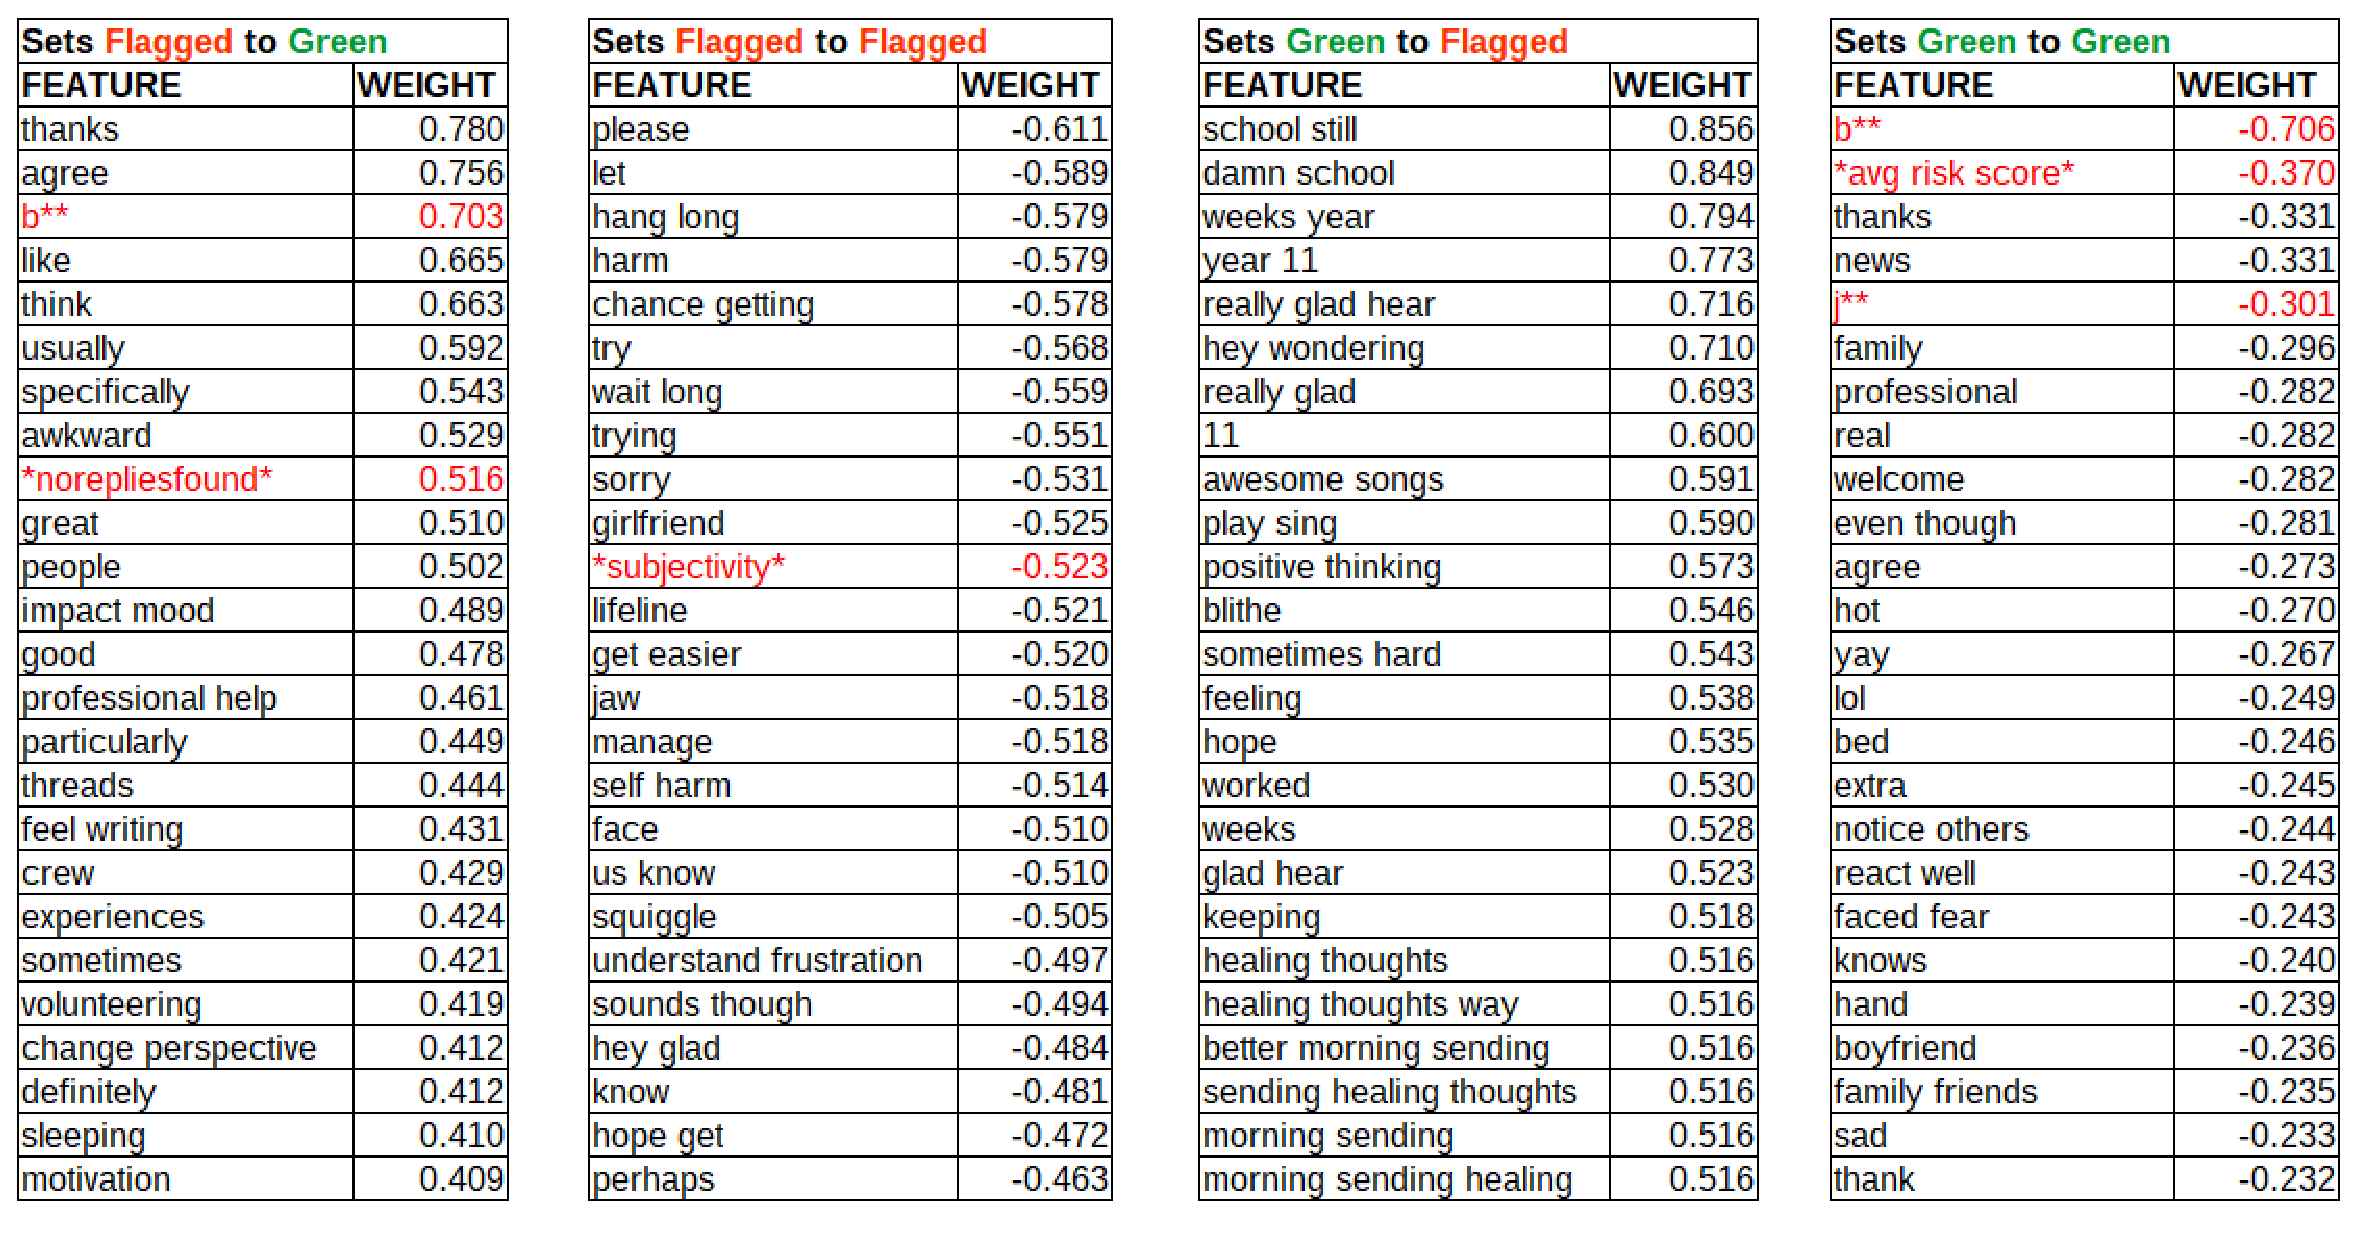
\includegraphics[width=16cm]{topfeatures}
    \caption{Highest/Lowest Weighted Features from Trained Models}
\end{figure}

\paragraph{Analysis}Our work on this task frequently generated new questions rather than answers, and we discuss the most significant remaining questions here.

\subparagraph{1. Are replies actually a factor that drive change in $U$'s state, or are they simply a reflection of $U$'s state?}We would like to be able to conclude that our top weighted features (for sets that move from a state of $flagged$ to $green$, for example) provide guidance to the ReachOut.com community about how to help a user in distress. The $flagged \rightarrow green$ top weighted terms receive a subjectivity score of 0.9 and positivity score of 0.9 using the NLTK sentiment analysis package, so they seem likely to influence $U$ in a positive way. The case with $flagged \rightarrow flagged$ top features is symmetical, having a polarity score of 0.9 and negativity score of 0.7. But causality is unclear, because the appearance of positive (negative) language is also exactly what we would expect to see in a conversation involving a $U$ with a positive (negative) attitude whose mental state is becoming more positive (negative). The top weighted terms from $green \rightarrow flagged$ actually get a positivity score of 0.7, so it is difficult to argue that the replies caused $U$'s distress to increase. There are many other explanations for the change in $U$'s mental state. Offline events likely have more influence than discussions on the forum. Some people might also be affected by simply thinking and writing about their feelings, regardless of any replies written to them (supported by the fact that our *norepliesfound* token was predictive of a $flagged$ $U$ turning $green$). Or people could be affected by passively reading other content on the forum that was not directed to them at all.

\subparagraph{2. Are some users more positively or negatively influential than others, or do they simply choose to participate on the forum in different ways?}This is similar to first question. Some usernames show up in our top weighted terms lists, and we would like to be able to conclude that those users are especially influential, and that their style of writing could serve as a model for what other users should do or not do. However, it is equally likely that some users simply choose to interact only with users or threads that have a positive tone. Others might focus on trying to help people who are suffering the most. We note that the two users who appear in Figure 4 (b** and j**) posted an above-average proportion of $flagged$ content (16-18\% vs. 7\% for the forum at large) despite appearing on the lists for $flagged \rightarrow green$ and $green \rightarrow green$.

\subparagraph{3. What is the effect of survivorship bias on our results?}It is important to note that we were able to construct only about 6,000 conversation sets for any value of $N$ (about 10,000 before removing the sets where $U$ was a moderator) when the dataset contained more than 65,000 posts. The difference is large because most of the time $U$ did not make a follow-up post, so we could not complete the set and add it to our training data. We cannot conclude anything about these users who stopped participating on the forum, and they might be the majority of users.

\section{Conclusion}

\paragraph{}With the set of features and classifier described in this paper, we can predict the change in an active ReachOut.com user's apparent mental state based on replies by other users in the community. However, there remains a lot of analysis and reasoning to be done before we can leverage the model to gain valuable insight into better helping users in distress. Specifically, we would like to see if there are certain words, phrases, or topics that bring a distressed user to a $green$ state, but the top terms we extract do not show a strong pattern; some make intuitive sense but some do not. Moreover, reasoning about causation is very difficult. Regardless, we believe that the ReachOut.com dataset remains valuable for this line of inquiry, and we hope that other researchers will take an interest and design better experiments to improve upon our results.

\begin{thebibliography}{9}

\bibitem{marchant}
Amanda Marchant,  Keith Hawton,  Ann Stewart,  Paul Montgomery,  Vinod Singaravelu,  Keith Lloyd,  Nicola Purdy,  Kate Daine,  Ann John. A Systematic Review of the Relationship Between Internet Use, Self-harm and Suicidal Behaviour in Young People: The Good, the Bad and the Unknown. PLOS ONE, 2017, retrieved from https://doi.org/10.1371/journal.pone.0181722
\bibitem{dunlop}
Sally M. Dunlop, Eian More, and Daniel Romer. Where do Youth Learn about Suicides on the Internet, and What Influence does this have on Suicidal Ideation? Journal of Child Psychology and Psychiatry 52:10, 2011, pages 1073-1080.
\bibitem{milne}
David N. Milne, Glen Pink, Ben Hachey, and Rafael A. Calvo. CLPsych 2016 Shared Task: Triaging Content in Online Peer-Support Forums. Proceedings of the Third Workshop on Computational Lingusitics and Clinical Psychology, 2016, pages 106-117.
\bibitem{phillips}
David P. Phillips. The Influence of Suggestion on Suicide: Substantive and Theoretical Implications of the Werther Effect. American Sociological Review, vol 39, No. 3, 1974, pages 340-354.
\bibitem{gladwell}
Malcolm Gladwell. The Tipping Point: How Little Things Can Make a Big Difference. New York: Little, Brown and Company Hachette Book Group, 2002. eBook Edition.
\bibitem{jonas}
Kai Jonas. Modelling and suicide: A test of the Werther effect. British Journal of Social Psychology, vol 31, 1992, pages 295-306.
\bibitem{ishii}
Keiko Ishii. Measuring mutual causation: Effects of suicide news on suicides in Japan. Social Science Research, vol 20, 1991, pages 188-195.
\bibitem{cheng}
Cheng ATA, Hawton K, Chen THH, Yen AMF, Chang JC, et al. The influence of media reporting of a celebrity suicide on suicidal behavior in patients with a history of depressive disorder. Journal of Affective Disorders, vol 103, 2007, pages 69-75.
\bibitem{sonneck}
Sonneck G, Etzersdorfer E, Nagel-Kuess S. Imitative suicide on the Viennese subway. Social Science and Medicine, vol 38, 1994, pages 453-457.
\bibitem{stack}
Steven Stack. Media Coverage as a Risk Factor in Suicide. Journal of Epidemiology \& Community Health 57.4, 2003, pages 238-240.
\bibitem{gould1}
Gould MS, Wallenstein S, Davidson L. Suicide clusters: A critical review. Suicide and Life-Threatening Behavior, vol 19, 1989, pages 17-29.
\bibitem{gould2}
Gould MS, Wallenstein S, Kleinman M. Time-space clustering of teenage suicide. American Journal of Epidemiology, vol 131, 1990, pages 71-78.
\bibitem{haw}
Haw CM. A cluster of suicides at a London psychiatric unit. Suicide and Life-Threatening Behavior, vol 24, 1994, pages 256-266.
\bibitem{brent}
Brent DA, Kerr MM, Goldstein C, Bozigar J, Wartella M, et al. An outbreak of suicide and suicidal behavior in a high school. Journal of the American Academy of Child \& Adolescent Psychiatry, vol 28, 1989, page 918.
\bibitem{kim}
Sunghwan Mac Kim, Yufei Wang, Stephen Wan, and Cecile Paris. Data61-CSIRO Systems at the CLPsych 2016 Shared Task. Proceedings of the Third Workshop on Computational Linguistics and Clinical Psychology, 2016.
\bibitem{cohan2}
Arman Cohan, Sydney Young, Andrew Yates, and Nazli Goharian. Triaging Content Severity in Online Mental Health Forums. arXiv preprint arXiv:1702.06875, 2017.
\bibitem{textblob}
``TextBlob is a Python (2 and 3) library for processing textual data. It provides a simple API for diving into common natural language processing (NLP) tasks such as part-of-speech tagging, noun phrase extraction, sentiment analysis, classification, translation, and more." https://textblob.readthedocs.io/en/dev/

\end{thebibliography}

\end{document}
